\documentclass[kravspec.tex]{subfiles}
\begin{document}
\section{Funktionelle krav}
Følgende funktionelle krav for systemet er blevet stillet: \\
\begin{enumerate}
	\item 
	\textbf{Real-time eye-tracking}: Systemet skal kunne foretage real-time eye-tracking.
	\item 
	\textbf{Kalibrering}: Før måling skal programmet kunne kalibreres.
	\item
	\textbf{Output}: Resultater af måling skal ende i en log-fil tilgængelig til brugeren.
	\item
	\textbf{Brugertilgang}: Ved hjælp af use case teknikken vil en yderlige række krav blive stillet. Disse vil lægge grundlag for bruger-program-interaktioner. Use-case-kravene er opstillet i afsnit \ref{usec}.  
\end{enumerate}

\subsection{Kalibrering}
Kalibrering: Specifikke ukendte variabler skal kunne kalibreres ved hjælp af interpolation. Herved skal programmet kunne tilpasses testpersonens fysiske forhold til kameraet. 
\begin{figure}[h]
\centering
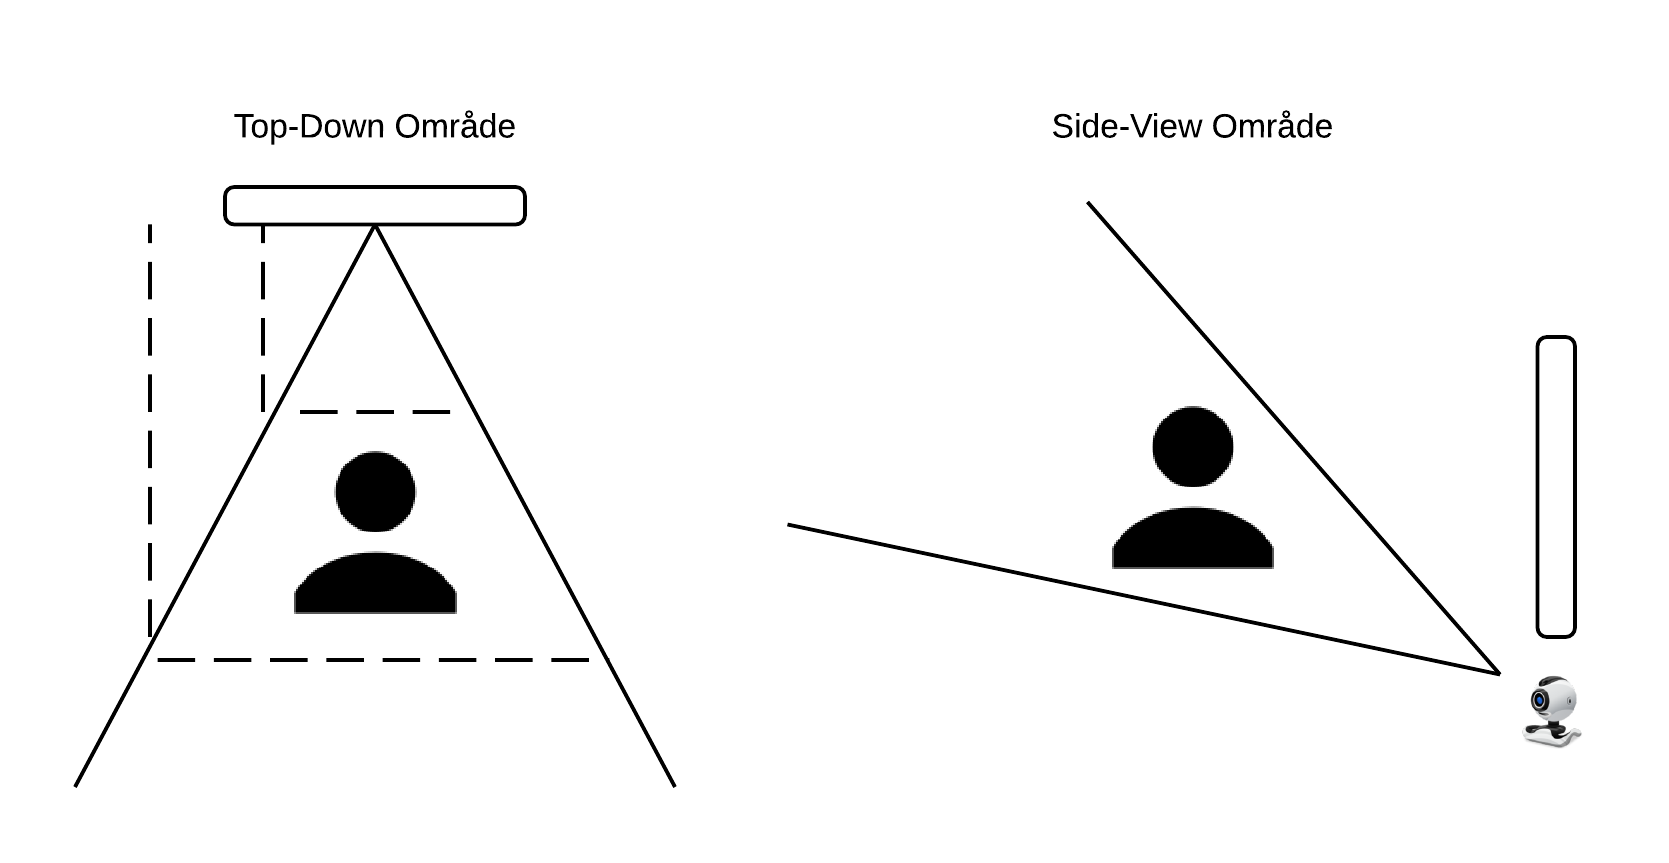
\includegraphics[width=0.7\linewidth]{../Kamera-testperson}
\caption{Kameraets position i forhold til testperson}
\label{fig:Camposition}
\end{figure}


Derudover skal programmet kunne kalibreres således at der kan findes tærskler (threshold-values) for trigger-niveauet: En værdi når trigger-niveauet går højt, og en værdi når trigger-niveauet går lavt.

\begin{figure}[H]
\centering
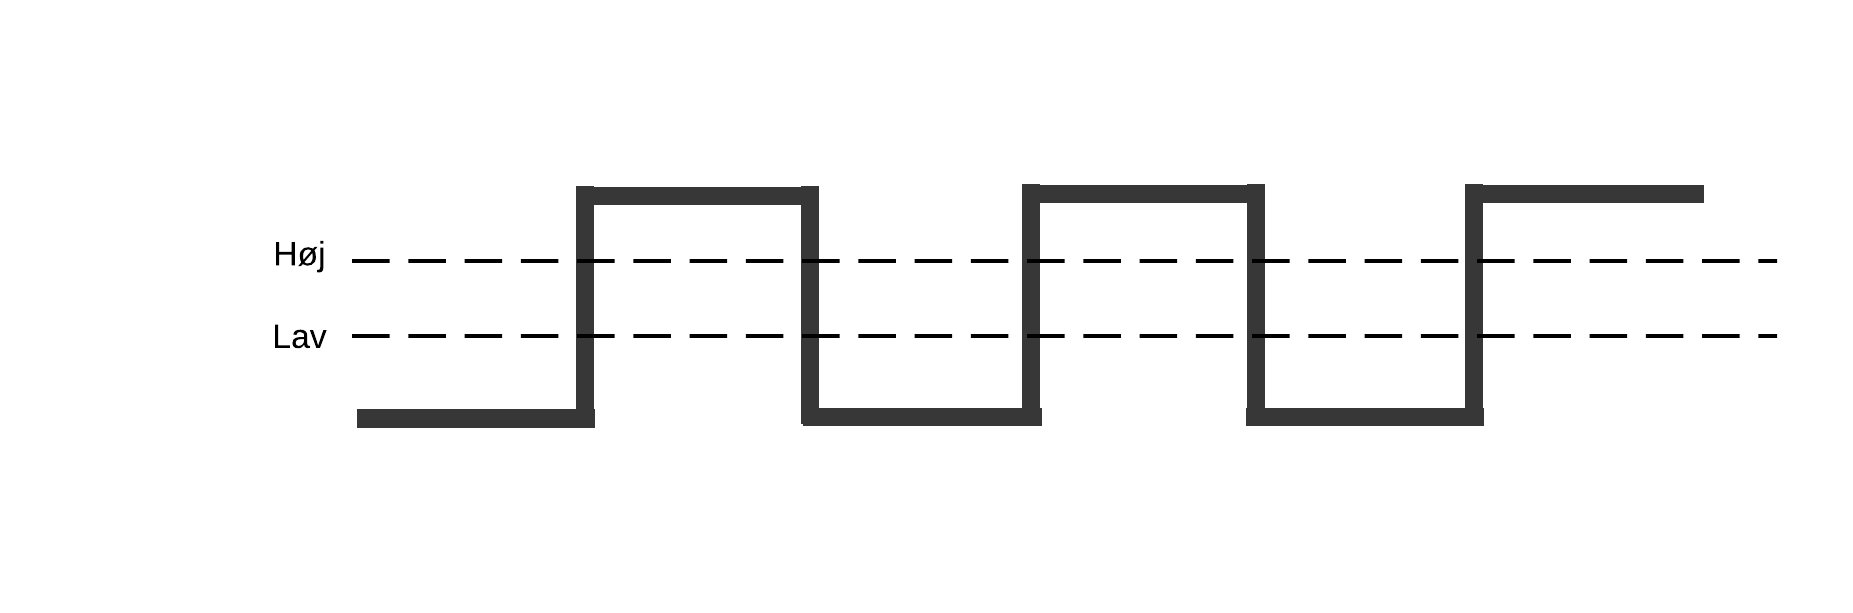
\includegraphics[width=0.7\linewidth]{../Trigger-threshold}
\caption{Eksempel på tærskelværdier for trigger-signalet}
\label{fig:Trigger-threshold}
\end{figure}



\subsection{Output}
For hver igangsat session skal programmet generere en log-fil med følgende data:
\indent \begin{itemize}

	\item 	Kommasepareret målingsdata med følgende format: \\
	\textit{X-koordinat, Y-koordinat, Samplenummer, Trigger-niveau (0 for lav, 1 for høj)} 
\end{itemize}

\subsection{Use-cases}	
\label{usec}
\begin{enumerate}
	\item Opret session: \\Opretter en session i en fil-sti med nødvendige data-filer. 
	\item Kalibrering: \\Initierer en række kalibreringer før brug. 
	\item Start måling: \\Igangsætter måling.
	\item Stop måling: \\Afslutter måling.
	\item Gem indstillinger: \\Gemmer en fil med brugerens nuværende indstillinger.
	\item Indlæs indstillinger: \\Indlæser indstillinger fra gemt fil.
	\item Indlæs rå data: \\Indlæser rå data fra tidligere session. 
\end{enumerate}


\end{document}